\subsection{Fundamental distributions}
The dominant background process is the $t\bar{t}$ production.
In the following, distributions of variables of simulated $t\bar{t}$ Monte Carlo events with muons are shown and compared to the expected distribution.
Some of these distriutions are shown in figure \ref{fig:distriutions}.
These are in agreement with the expected distributions of these variables.
In figure \ref{fig:btagged}, the number of b-tagged jets in each event is shown.
Figure \ref{fig:decay} shows the production of two bottom quarks so that most likely two jets are b-tagged.
This expectation is in agreement with figure \ref{fig:btagged}.
The remaining momentum that is not in the jets is evenly split on the muon and the neutrino.
The distributions of the $\texttt{lep$\_$pt}$ and $\texttt{met$\_$et}$ is very similar.
Both have their respective peak at the same location.
The $\texttt{met$\_$et}$ is more smeared out since the indirect measured neutrinos have a worse resolution.
Besides that these variables follow their expected distributions.

\begin{figure}
  \begin{subfigure}{0.5\textwidth}
    \centering
    \includegraphics[width=\linewidth]{plots/ttbar.mu_selected_lep_pt.pdf}
    \caption{}
    \label{fig:lep_pt}
  \end{subfigure}%
  \begin{subfigure}{0.5\textwidth}
    \centering
    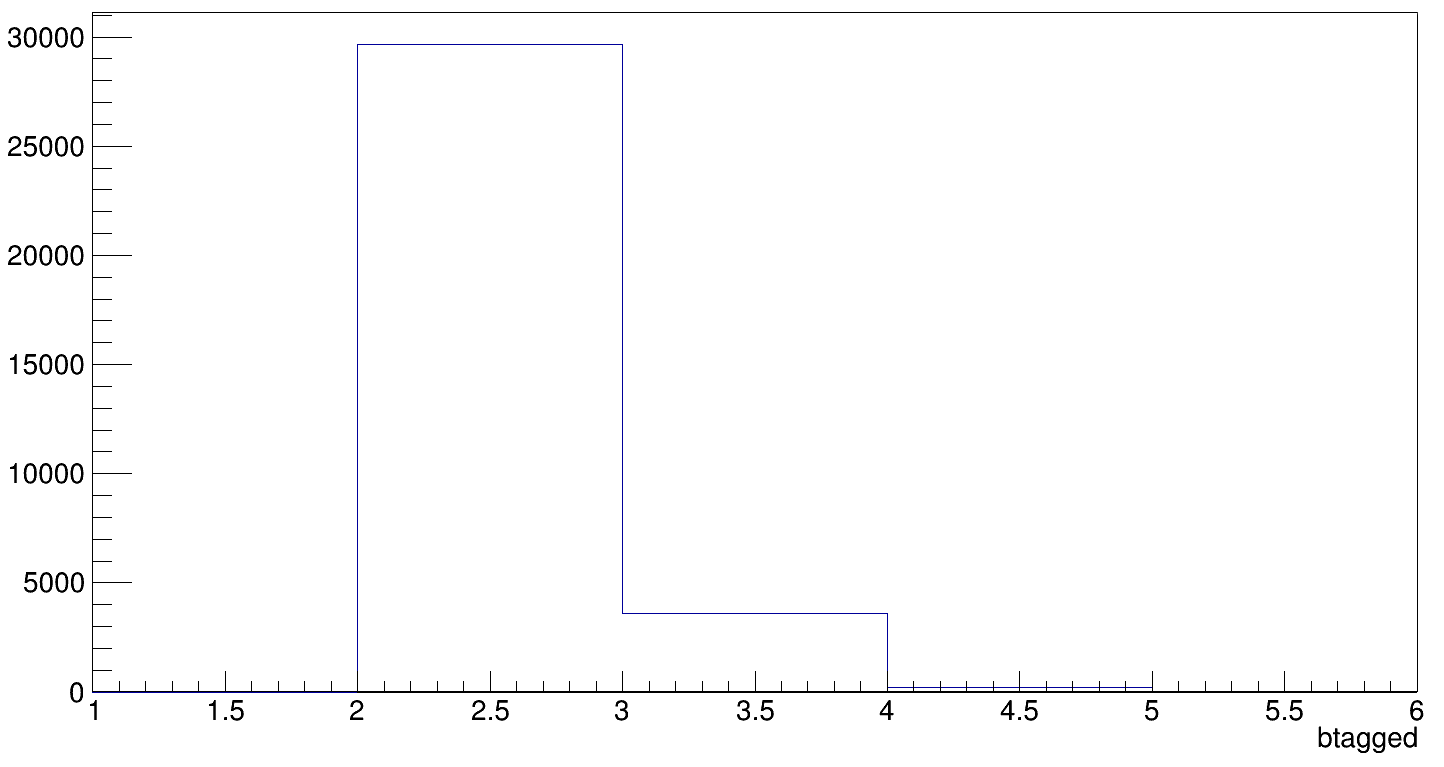
\includegraphics[width=\linewidth]{plots/btagged.png}
    \caption{}
    \label{fig:btagged}
  \end{subfigure}%
  \newline
  \begin{subfigure}{0.5\textwidth}
    \centering
    \includegraphics[width=\linewidth]{plots/ttbar.mu_selected_jet_pt.pdf}
    \caption{}
    \label{fig:jet_pt}
  \end{subfigure}%
  \begin{subfigure}{0.5\textwidth}
    \centering
    \includegraphics[width=\linewidth]{plots/ttbar.mu_selected_met_et.pdf}
    \caption{}
    \label{fig:met_et}
  \end{subfigure}%
  \caption{Plots of different variables of the $t\bar{t}$ Monte Carlo simulations.
  The following variables are shown here: The transversal momentum of the lepton (\subref{fig:lep_pt}), the amount of b-tagged jets (\subref{fig:btagged}), the transversal momentum of the jets (\subref{fig:jet_pt}) and the missing transversal energy (\subref{fig:met_et}).
  }
  \label{fig:Distributions}
\end{figure}

\subsection{Derived quantities}

After the event selection, some background processes like $t\bar{t}$ events are still not negligible.
To have a better discrimination, some quantities are being computed that might increase the seperation power between $Z^\prime$ and $t\bar{t}$ events. The following quantities were computed and compared in $Z^\prime$ and $t\bar{t}$ events:
\begin{itemize}
 \item the difference of the azimuth angle of the missing transversal energy and the lepton flight direction $\Delta\Phi$
 \item the invariant mass of the system formed by the three jets with the largest transversal momentum
 \item the invariant mass and the pseudorapidity of the system formed by the four jets with the largest momentum, the muon and the neutrino
\end{itemize}
To calculate the invariant mass of the system including neutrinos, the class \texttt{TLorentzVektor} was used to compute the four-vector information.
While calculating $\Delta\Phi$, only the smaller difference of $|\phi_1 - \phi_2|$ and $|2\pi - |\phi_1 - \phi_2|$ was used.
These quantities were calculated for all data and Monte Carlo samples.
To determine the quantity with the largest separation power, the dominant background ($t\bar{t}$) is compared with a possible signal ($Z^\prime(1000)$).
The best discriminate is the invariant mass of the full system.
This quantity is shown in figure \ref{fig:Comparison} for $t\bar{t}$ and $Z^\prime(1000)$.

\begin{figure}
  \begin{subfigure}{0.5\textwidth}
    \centering
    \includegraphics[width=\linewidth]{plots/ttbar.mu_selected_SysJetMass.pdf}
    \caption{}
    \label{fig:ttbar_sys}
  \end{subfigure}%
  \begin{subfigure}{0.5\textwidth}
    \centering
    \includegraphics[width=\linewidth]{plots/zprime1000.mu_selected_SysJetMass.pdf}
    \caption{}
    \label{fig:zprime_sys}
  \end{subfigure}%
  \caption{Distribution of the chosen discrimination quantity, the invariant mass of the system formed by the four jets with the largest transversal momentum, the muon and the neutrino.
This quantity is shown for $t\bar{t}$ simulations (\subref{fig:ttbar_sys}) and simulations of  $Z^\prime(1000)$ (\subref{fig:zprime_sys}).
  }
  \label{fig:Comparison}
\end{figure}
